\section{Veränderungen}
\subsection{Klassendiagramm}
Im Folgenden wird anhand des aktualisierten Klassendiagramms gezeigt, was sich zum Entwurf verändert hat.

%altes klassendiagramm

In der view haben sich folgenden Änderungen ergeben:

In der conrtol haben sich folgende Änderungen ergeben:

Im model haben sich folgende Änderungen ergeben: %TODO tex syntax

Daraus ergibt sich das aktualisierte Klassendiagramm:

%neues Klassendiagramm

\subsection{Sequenzen}
Die Sequenzdiagramme aus dem Entwurfen haben sich wie folgt verändert:
\subsubsection{Login Sequenz}

\begin{figure}
  \centering
    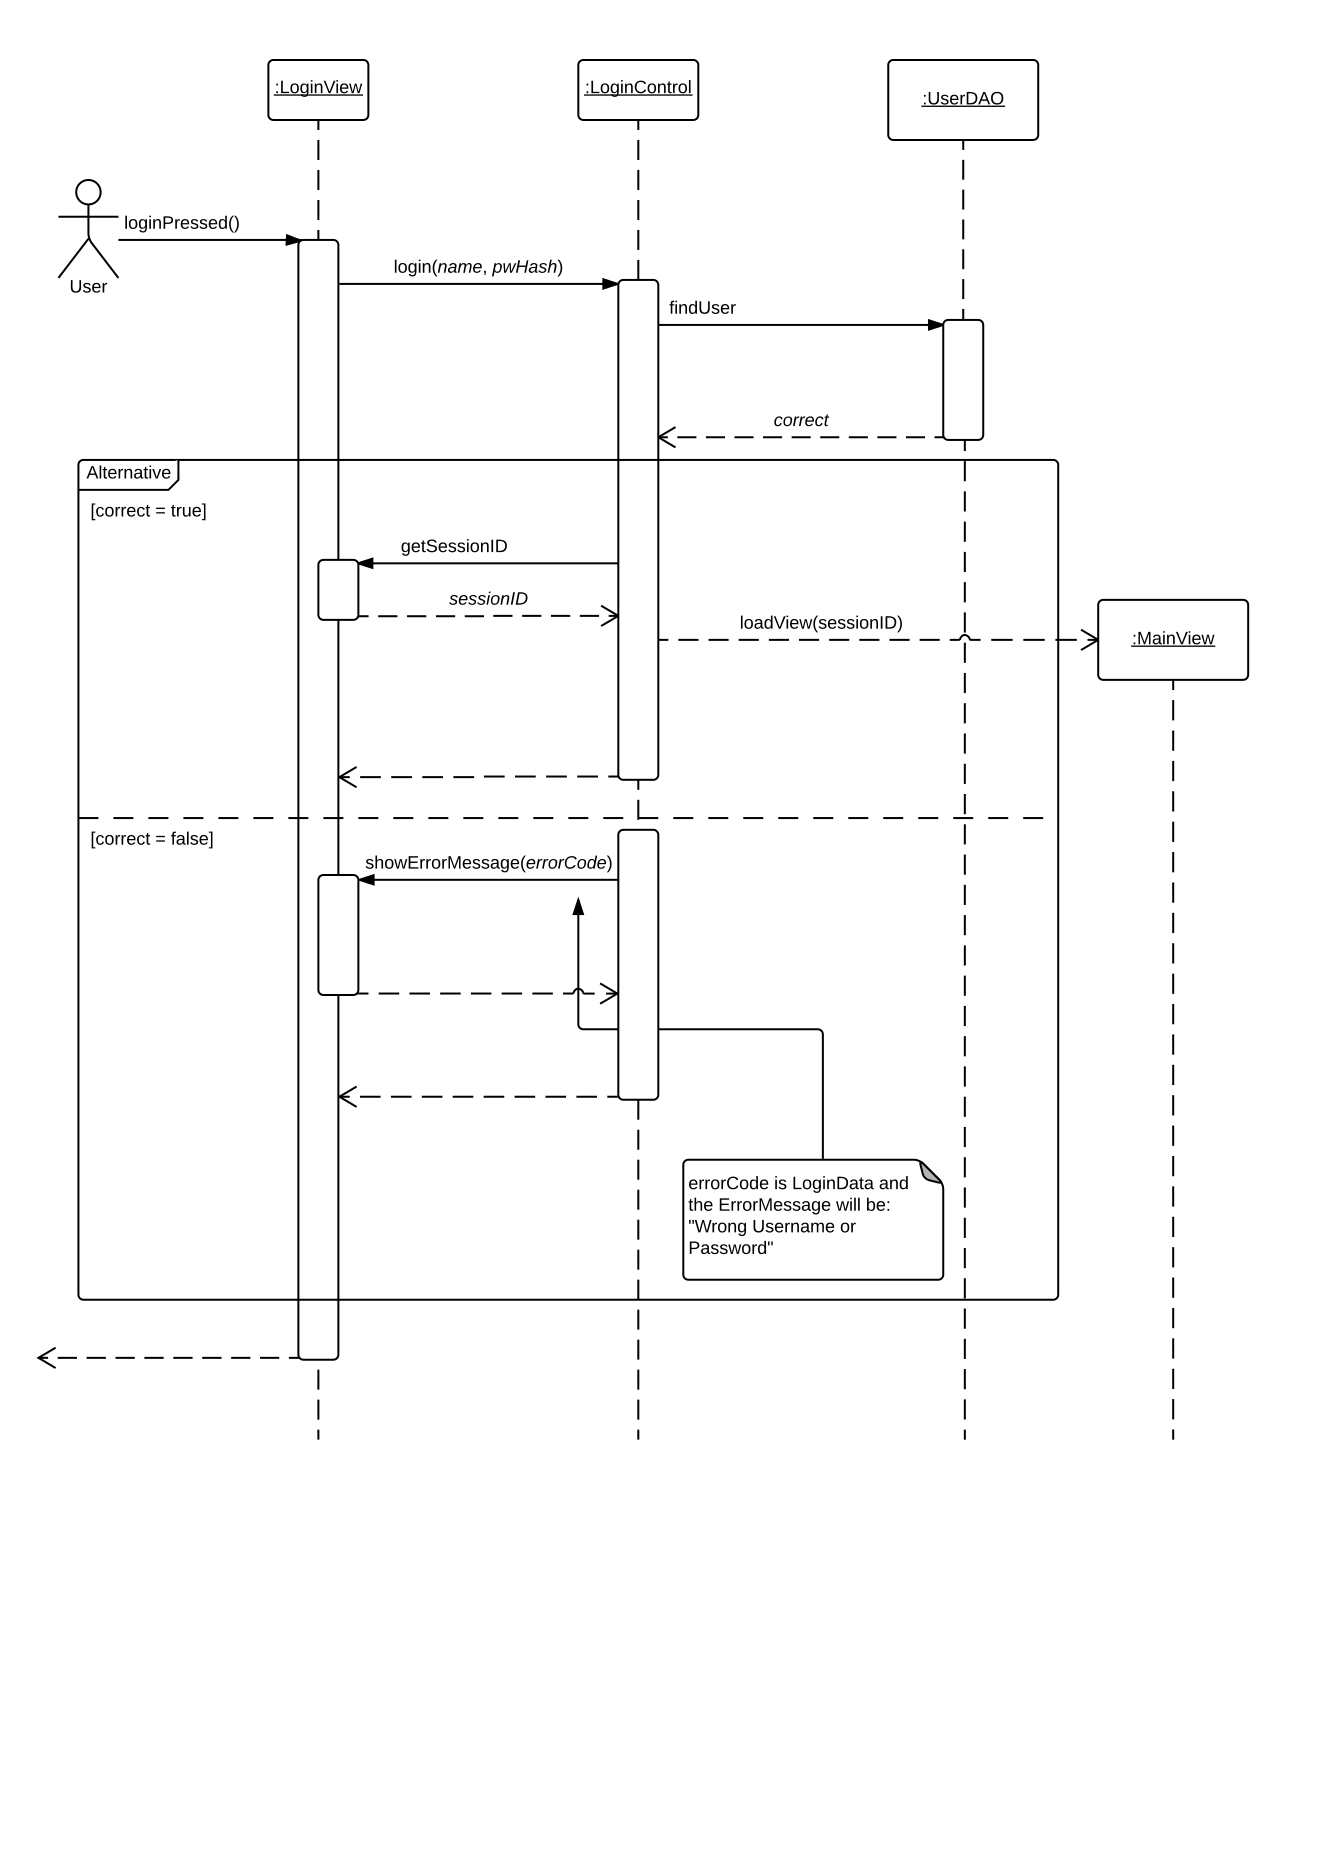
\includegraphics[width=\linewidth]{Login-Sequenz.svg}
   \caption{Alte Login Sequenz}
\end{figure}

\paragraph{Veränderungen}
\begin{itemize}
    \item Login wurde um die Funktion \emph{remember me} erweitert.
    \item Die Authentifizierung wurde in einklang mit dem Shiro Framework gestaltet:
    \begin{itemize}
        \item Zum Login wird ein token aus Passwort und Username genutzt.
        \item Durch das Token wird der Nutzer ermittelt und dessen Authentifizierungsdaten\(Password, ...\) geholt.
        \item Diese werden mittels einen speziellen Hash vergleicher mit dem angegebenen Token verglichen.
    \end{itemize}
    \item Laden der View wurde durch Vaadins \emph{navigateTo} ersetzt.
\end{itemize}

\begin{figure}
  \centering
    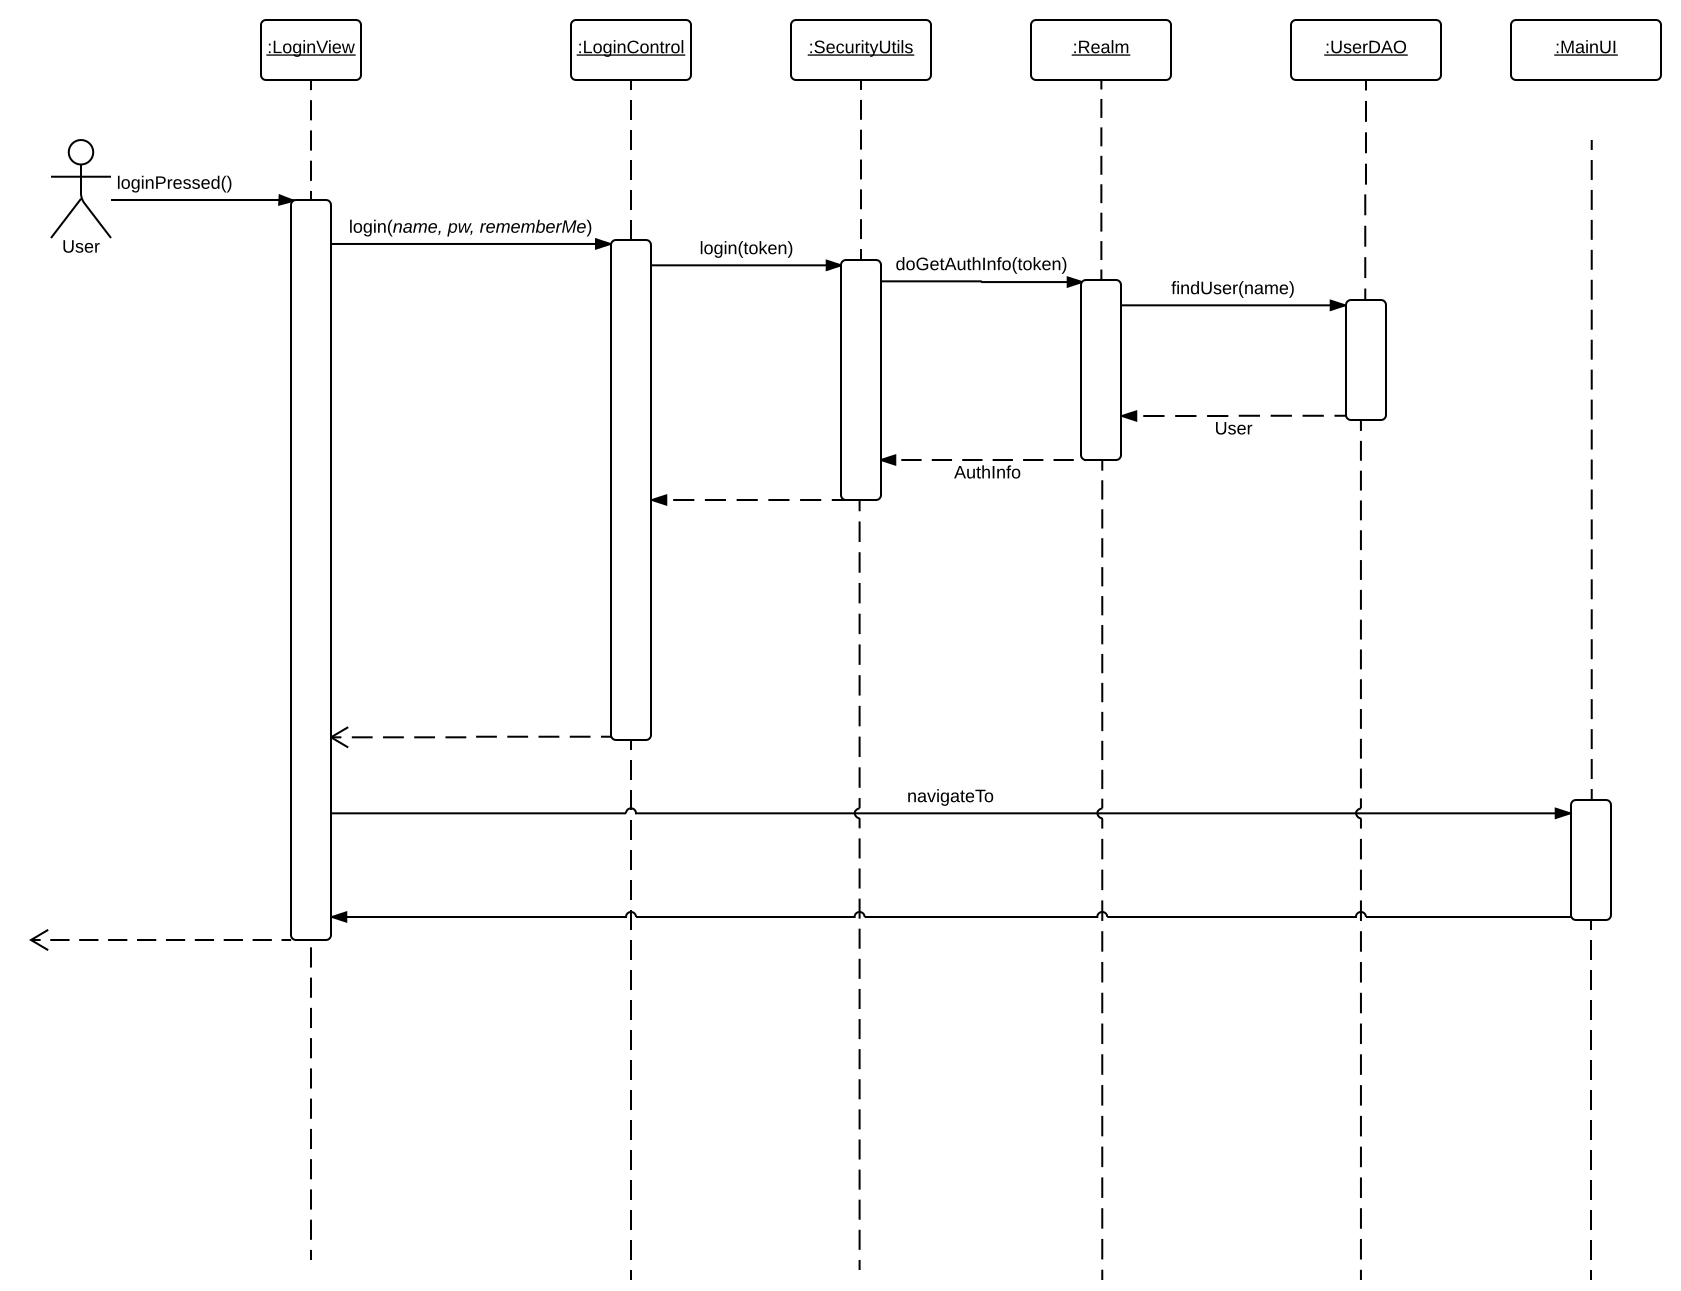
\includegraphics[width=\linewidth]{Login-Sequenz-new.svg}
   \caption{Neue Login Sequenz}
\end{figure}

\subsection{Account erstellungs sequenz}

\begin{figure}
  \centering
    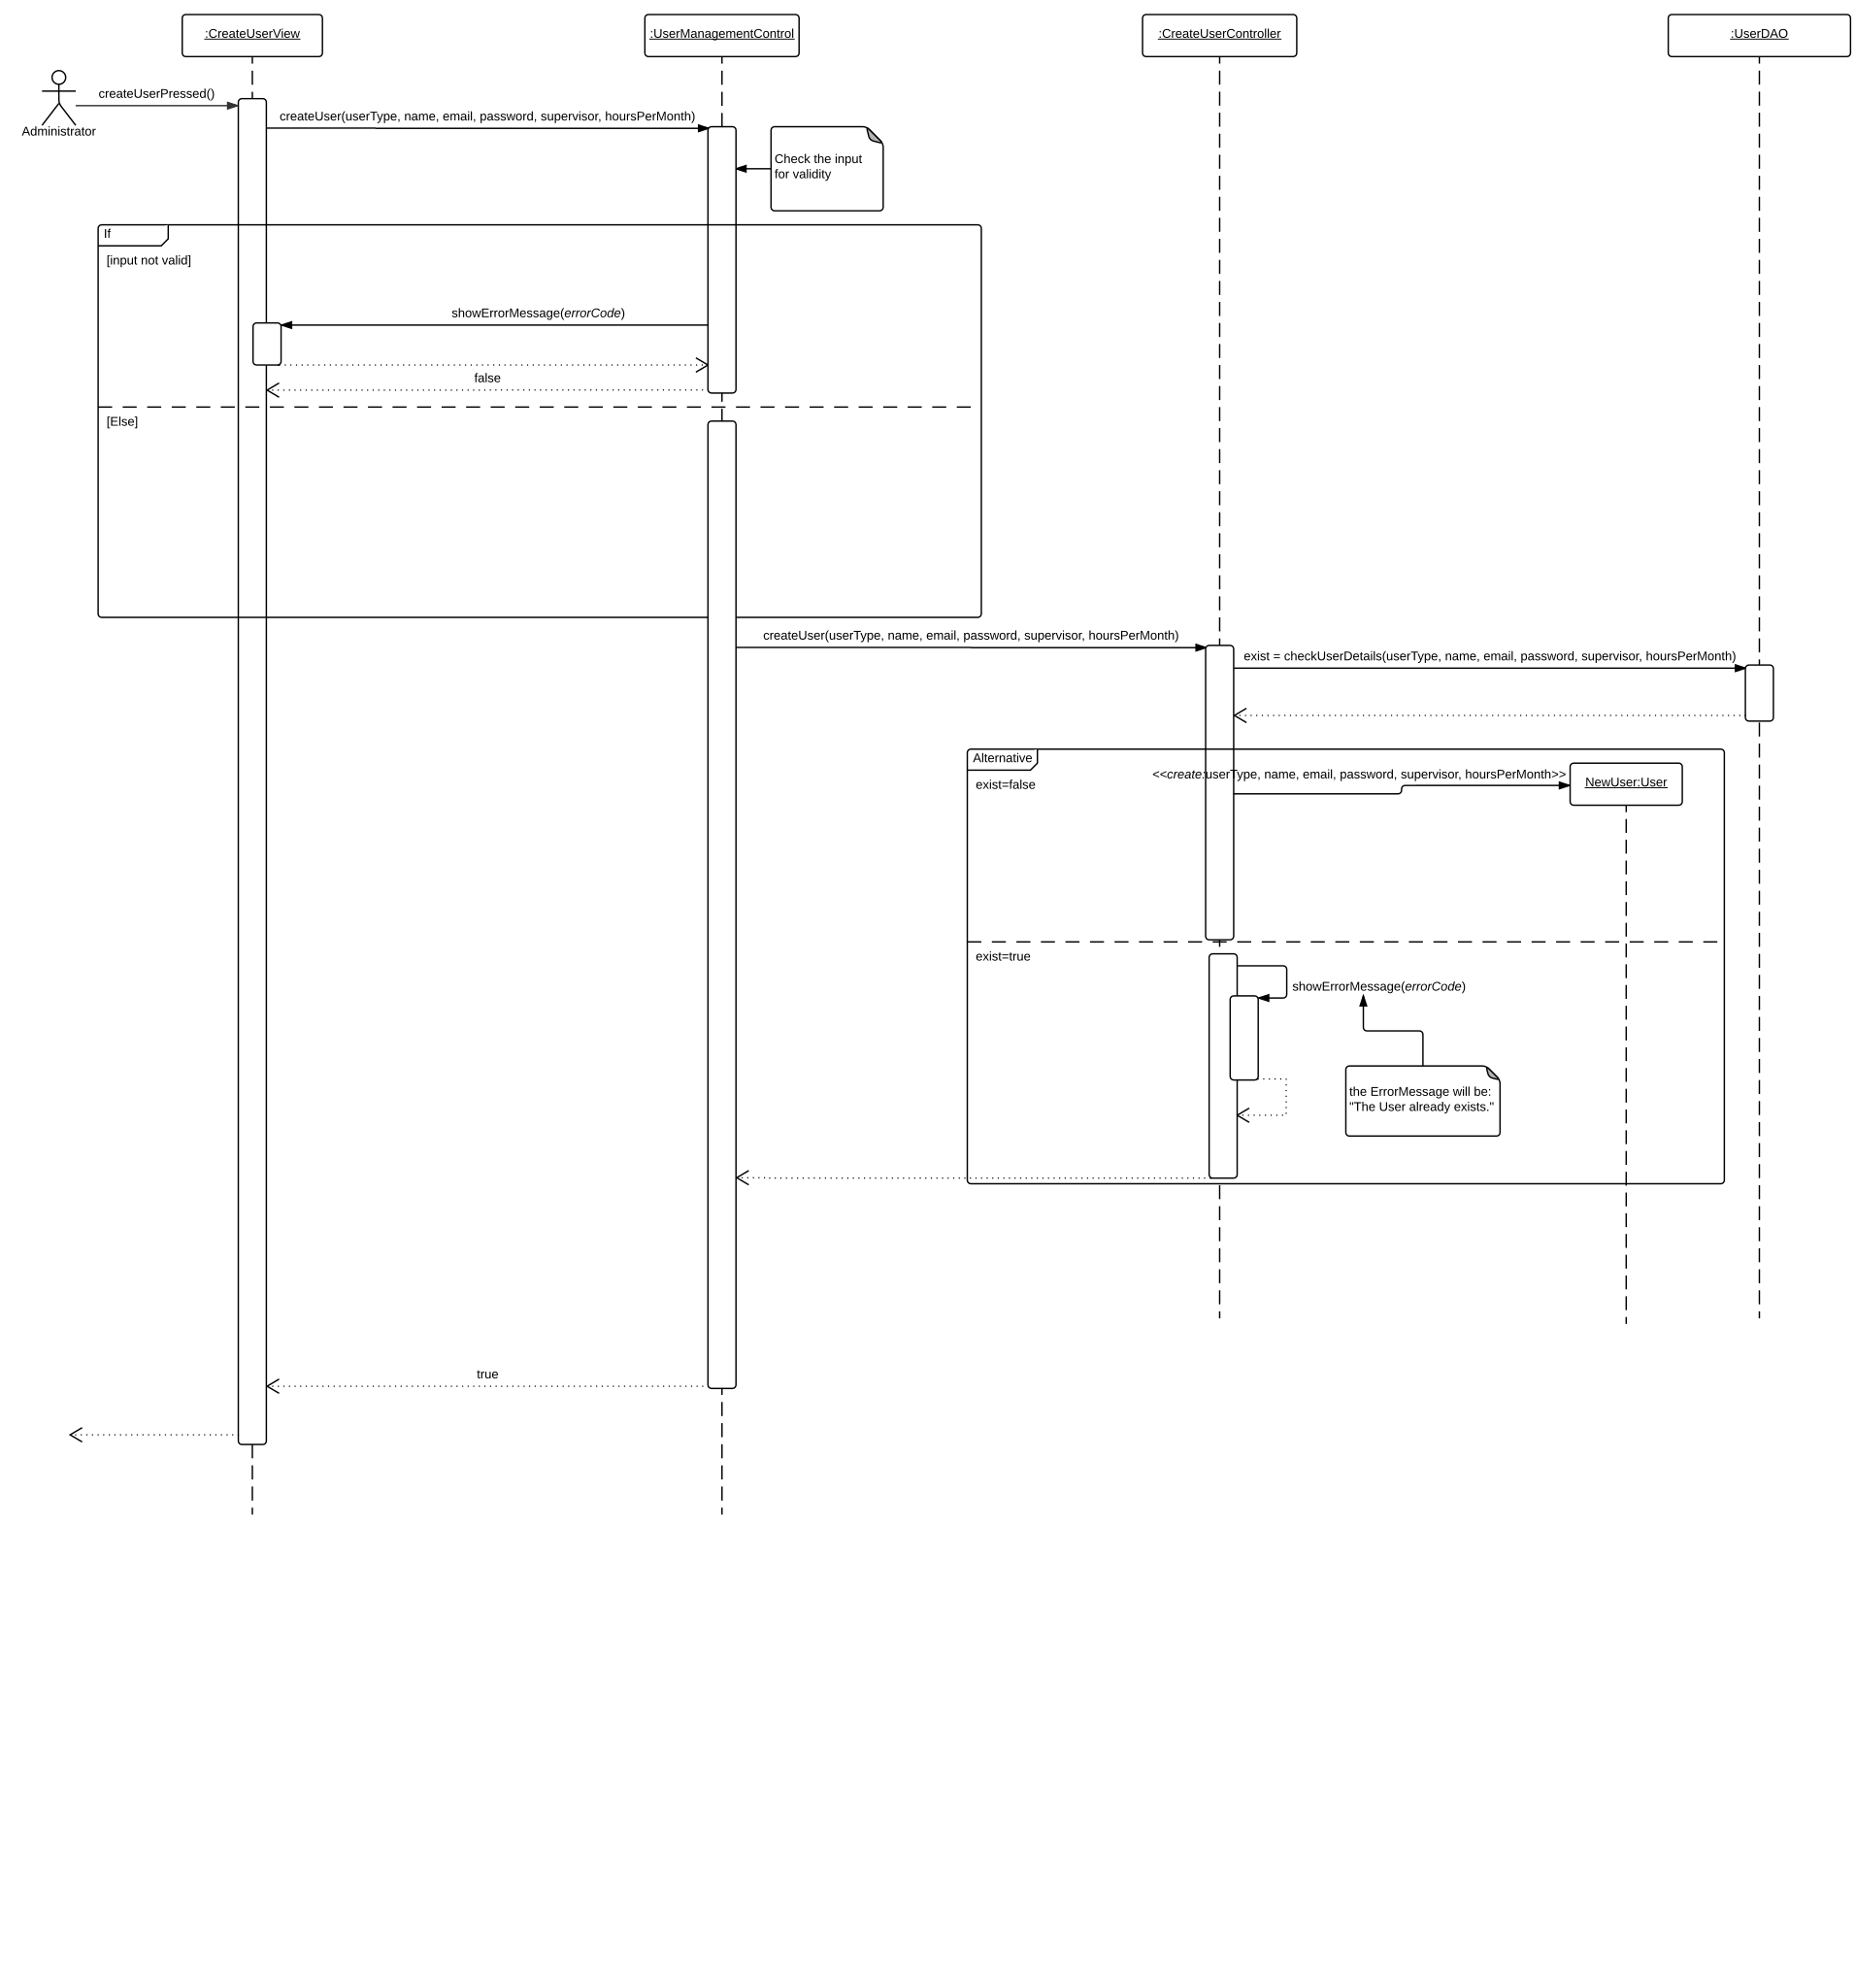
\includegraphics[width=\linewidth]{Create-user-account.svg}
   \caption{Alte Login Sequenz}
\end{figure}

\paragraph{Veränderungen}
\begin{itemize}
    \item Der Ablauf wurde vereinfacht. Es wird nurnoch die CreateUserControl Klasse angespochen.
    \item Überprüfungen wurden durch eine verbesserte klarere interne Exception Struktur vereinfacht.
\end{itemize}

\begin{figure}
  \centering
    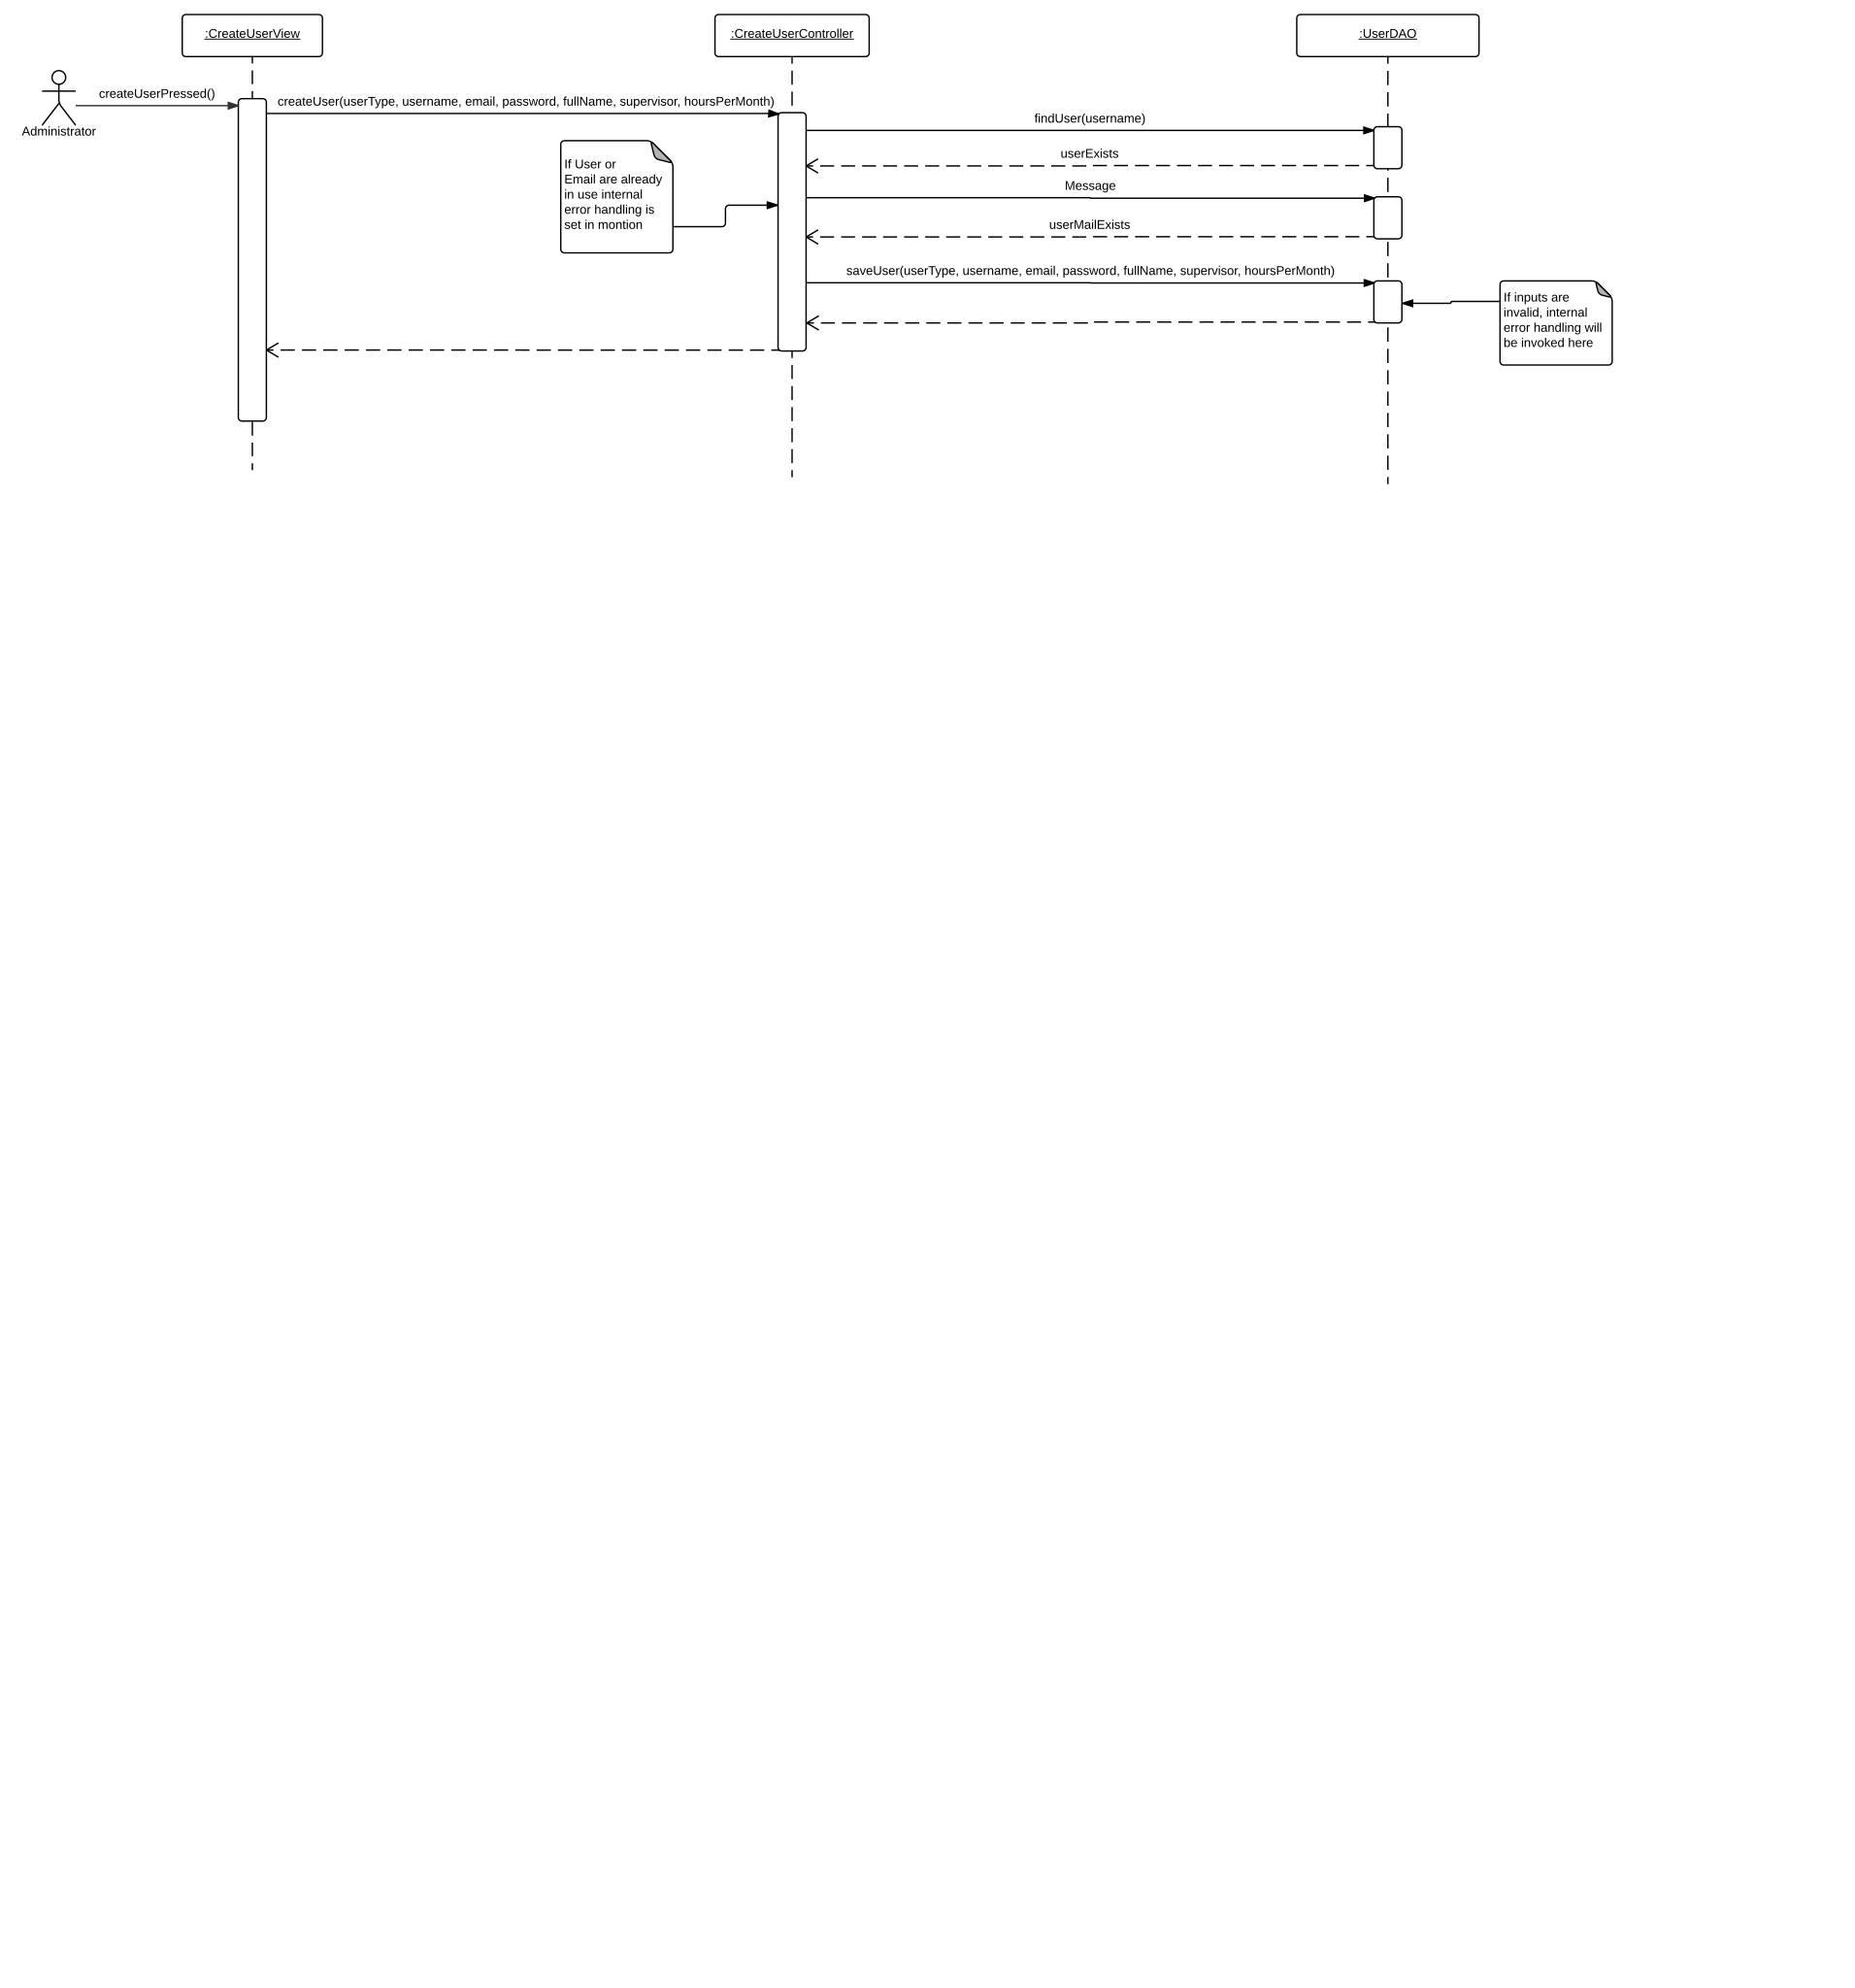
\includegraphics[width=\linewidth]{Create-user-account-new.svg}
   \caption{Alte Login Sequenz}
\end{figure}